% The prism identity: g(sigma) - f(sigma) = partial_Y(P_n sigma) + P_{n-1}(partial_X sigma).
% Source: book/tex/homology/singular.tex (§ Geometry of chain complexes).
\documentclass[border=2mm]{standalone}
\usepackage{tikz}
\usepackage{amsmath}
\usetikzlibrary{arrows.meta}
\definecolor{heavygreen}{rgb}{0,0.5,0}
\begin{document}
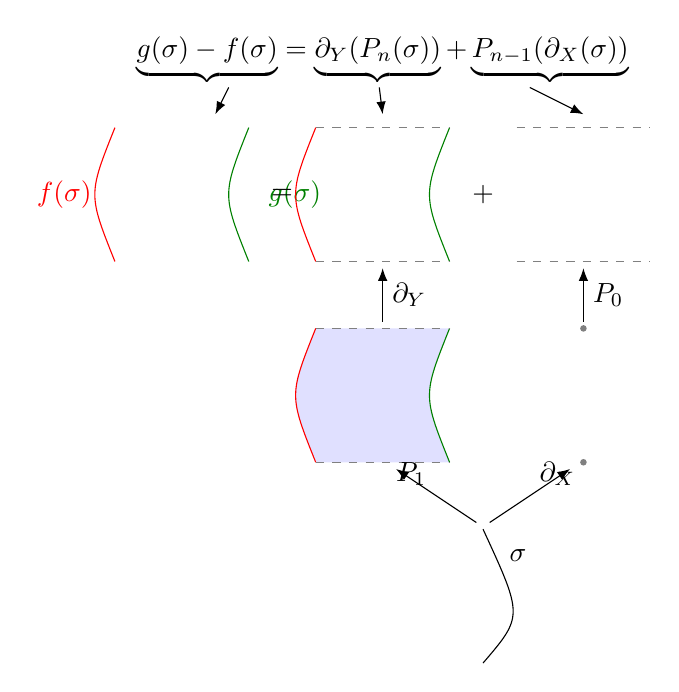
\begin{tikzpicture}[>={Latex[length=1.6mm]}, scale=0.85]
  \node at (4,9) {$\underbrace{g(\sigma) - f(\sigma)}
    = \underbrace{\partial_Y(P_n(\sigma))}
    + \underbrace{P_{n-1}(\partial_X(\sigma))}$};
  \draw[->] (1.7,8.6)--(1.5,8.2);
  \draw[->] (3.95,8.6)--(4,8.2);
  \draw[->] (6.2,8.6)--(7,8.2);
  % term 1: g - f
  \draw[red] (0,8) .. controls (-0.4,7) .. (0,6);
  \node[red,left] at (-0.2,7) {$f(\sigma)$};
  \draw[heavygreen] (2,8) .. controls (1.6,7) .. (2,6);
  \node[heavygreen,right] at (2.15,7) {$g(\sigma)$};
  \node at (2.5,7) {$=$};
  % term 2: prism, top row
  \draw[red] (3,8) .. controls (2.6,7) .. (3,6);
  \draw[heavygreen] (5,8) .. controls (4.6,7) .. (5,6);
  \draw[gray,dashed] (3,8)--(5,8);
  \draw[gray,dashed] (3,6)--(5,6);
  \node at (5.5,7) {$+$};
  % term 3: grey top/bottom
  \draw[gray,dashed] (6,8)--(8,8);
  \draw[gray,dashed] (6,6)--(8,6);
  % lower: filled prism with partial_Y
  \fill[blue!12] (3,5) .. controls (2.6,4) .. (3,3) -- (5,3) .. controls (4.6,4) .. (5,5) -- cycle;
  \draw[red] (3,5) .. controls (2.6,4) .. (3,3);
  \draw[heavygreen] (5,5) .. controls (4.6,4) .. (5,3);
  \draw[gray,dashed] (3,5)--(5,5);
  \draw[gray,dashed] (3,3)--(5,3);
  \draw[->] (4,5.1)--(4,5.9); \node[right] at (4,5.5) {$\partial_Y$};
  % lower right: P_0 dots
  \fill[gray] (7,3) circle (1.4pt); \fill[gray] (7,5) circle (1.4pt);
  \draw[->] (7,5.1)--(7,5.9); \node[right] at (7,5.5) {$P_0$};
  % bottom: sigma with P_1 and partial_X
  \draw (5.5,0) .. controls (6.1,0.7) .. (5.5,2); \node[right] at (5.75,1.6) {$\sigma$};
  \draw[->] (5.4,2.1)--(4.2,2.9); \node[above left] at (4.8,2.5) {$P_1$};
  \draw[->] (5.6,2.1)--(6.8,2.9); \node[above right] at (6.2,2.5) {$\partial_X$};
\end{tikzpicture}
\end{document}
